\begin{task}
Oblicz moc sygnału okresowego $f(t)$ przedstawionego na rysunku 

\begin{figure}[H]
\centering
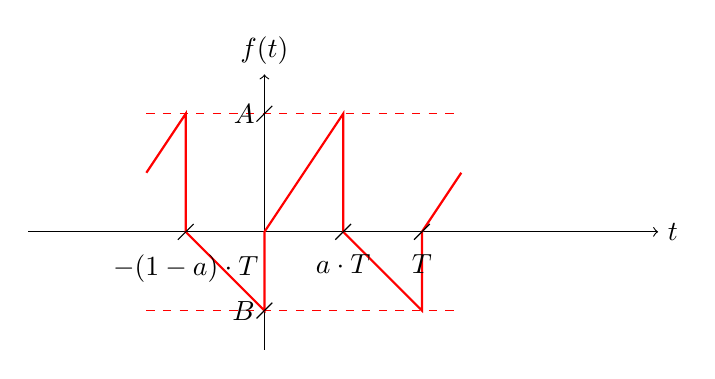
\begin{tikzpicture}
  %\draw (0,0) circle (1in);
  \draw[->] (-3.0,+0.0) -- (+5.0,+0.0) node[right] {$t$};
  \draw[->] (+0.0,-1.5) -- (+0.0,+2.0) node[above] {$f(t)$};
  \draw[-,red, thick] (-1.5,0.75) -- (-1.0,1.5)--(-1.0,0.0) -- (0.0,-1.0) -- (0.0,+0.0) -- (+1.0,+1.5) -- (+1.0,+0.0) -- (+2.0,-1.0) -- (+2.0,+0.0) -- (2.5,0.75);
  \draw[-,red, dashed] (-1.5,1.5) -- (2.5,1.5);
  \draw[-,red, dashed] (-1.5,-1.0) -- (2.5,-1.0);
  %\draw[-] (-1.0-0.1,-0.1)--(-1.0+0.1,0.1) node[midway, below, outer sep=10pt,align=center] {$-\frac{T}{2}$};
  \draw[-] (-1.0-0.1,-0.1)--(-1.0+0.1,0.1) node[midway, below, outer sep=5pt] {$-(1-a)\cdot T$};
  \draw[-] (+1.0-0.1,-0.1)--(+1.0+0.1,0.1) node[midway, below, outer sep=5pt] {$a\cdot T$};
  \draw[-] (+2.0-0.1,-0.1)--(+2.0+0.1,0.1) node[midway, below, outer sep=5pt] {$T$};
  \draw[-] (-0.1,+1.5-0.1)--(+0.1,+1.5+0.1) node[midway, left] {$A$};
  \draw[-] (-0.1,-1.0-0.1)--(+0.1,-1.0+0.1) node[midway, left] {$B$};

\end{tikzpicture}
\end{figure}

W pierwszej kolejności należy ustalić wzór funkcji przedstawionej na rysunku.
Jest to funkcja odcinkowa. W pierwszym okresie możemy ją opisać za pomocą dwóch prostych.
Ogólne równanie prostej:

\begin{equation}
f(t) = m \cdot t + b
\end{equation}

W pierwszym okresie, w pierwszej części, wykres funkcji jest prostą przechodzącą przez dwa punkty: $(0,0)$ oraz $(a\cdot T,A)$. Możemy więc napisać układ równań rozwiązać go i znaleźć nie znane parametry $m$ i $b$.  

\begin{align*}
&\left\{\begin{matrix*}[l]
0 = m\cdot 0 +b\\ 
A = m\cdot a \cdot T +b
\end{matrix*}\right. \\
&\left\{\begin{matrix*}[l]
0 = b\\ 
A = m \cdot a\cdot T +b
\end{matrix*}\right. \\
&\left\{\begin{matrix*}[l]
0 = b\\ 
A = m \cdot a\cdot T +0
\end{matrix*}\right. \\
&\left\{\begin{matrix*}[l]
0 = b\\ 
\frac{A}{a\cdot T} = m
\end{matrix*}\right.
\end{align*}
Podsumowując, pierwszy odcinek funkcji przedstawionej na rysunku, w pierwszym okresie można opisać wzorem:
\begin{align*}
f(t) = \frac{A}{a \cdot T}\cdot t
\end{align*}

Drugi odcinek funkcji jest prostą przechodzącą przez następujące dwa punkty: $(a \cdot T,0)$ oraz $(T,-B)$. Możemy więc napisać układ równań rozwiązać go i znaleźć nie znane parametry $m$ i $b$.

\begin{align*}
&\left\{\begin{matrix*}[l]
0 = m\cdot a \cdot T +b\\ 
-B = m\cdot T +b
\end{matrix*}\right. \\
&\left\{\begin{matrix*}[l]
-m \cdot a \cdot T = b\\ 
-B = m \cdot T -m \cdot a \cdot T
\end{matrix*}\right. \\
&\left\{\begin{matrix*}[l]
-m \cdot a \cdot T = b\\ 
-B = m \cdot \left( T - a \cdot T\right)
\end{matrix*}\right. \\
&\left\{\begin{matrix*}[l]
-m \cdot a \cdot T = b\\ 
-\frac{B}{T - a \cdot T} = m
\end{matrix*}\right. \\
&\left\{\begin{matrix*}[l]
\frac{B}{T - a \cdot T} \cdot a \cdot T = b\\ 
-\frac{B}{T - a \cdot T} = m
\end{matrix*}\right. \\
&\left\{\begin{matrix*}[l]
\frac{B}{1 - a} \cdot a = b\\ 
-\frac{B}{T - a \cdot T} = m
\end{matrix*}\right.
\end{align*}
A więc drugi odcinek funkcji przedstawionej na rysunku w pierwszym okresie, można opisać wzorem:
\begin{align*}
f(t) = -\frac{B}{T - a \cdot T}\cdot t + \frac{B}{1 - a} \cdot a
\end{align*}
W związku z tym całą funkcję w pierwszym okresie można zapisać jako funkcje przedziałową:
\begin{align*}
f(t) = \left\{\begin{matrix*}[l]
\frac{A}{a \cdot T}\cdot t & dla &t \in (0; a \cdot T)\\ 
-\frac{B}{T - a \cdot T}\cdot t + \frac{B}{1 - a} \cdot a & dla & t \in (a \cdot T; T)
\end{matrix*}\right.
\end{align*}
I ogólniej całą funkcję można wyrazić następującym wzorem:
\begin{align*}
f(t) = \left\{\begin{matrix*}[l]
\frac{A}{a \cdot T}\cdot \left( t - k\cdot T \right) & dla &t \in (0 + k\cdot T; a \cdot T + k\cdot T)\\ 
-\frac{B}{T - a \cdot T}\cdot \left( t - k\cdot T \right) + \frac{B}{1 - a} \cdot a & dla & t \in (a \cdot T+ k\cdot T; T+ k\cdot T)
\end{matrix*}\right. \wedge k \in C
\end{align*}

Moc sygnału okresowego wyznaczamy z wzoru
\begin{equation}
P=\frac{1}{T} \cdot \int_{T}^{}\left|f(t)\right|^2 \cdot dt
\end{equation}
Podstawiamy do wzoru na moc wzór naszej funkcji
%\begin{equation}
%\begin{aligned}
\begin{align*}
P&=\frac{1}{T} \cdot \int_{T}^{}\left|f(t)\right|^2 \cdot dt=\\
 &=\frac{1}{T} \cdot \left( \int_{0}^{a \cdot T}\left|\frac{A}{a \cdot T}\cdot t \right|^2 \cdot dt
  +\int_{a \cdot T}^{T}\left|\frac{B}{T - a \cdot T}\cdot t - \frac{B}{1 - a} \cdot a\right|^2 \cdot dt \right)=\\ 
 &=\frac{1}{T} \cdot \int_{0}^{a \cdot T}\left(\frac{A}{a \cdot T}\cdot t \right)^2 \cdot dt
  +\frac{1}{T} \cdot \int_{a \cdot T}^{T}\left(\frac{B}{T - a \cdot T}\cdot t - \frac{B}{1 - a} \cdot a\right)^2 \cdot dt=\\ 
 &=\frac{1}{T} \cdot \int_{0}^{a \cdot T}\frac{A^2}{a^2 \cdot T^2}\cdot t^2 \cdot dt
 +\frac{1}{T} \cdot \int_{a \cdot T}^{T}\left(\left(\frac{B}{T - a \cdot T}\cdot t\right)^2 - 2\cdot \frac{B}{T - a \cdot T}\cdot t \cdot  \frac{B}{1 - a} \cdot a + \left( \frac{B}{1 - a} \cdot a\right)^2 \right) \cdot dt=\\
 &=\frac{A^2}{a^2 \cdot T^3}\cdot \int_{0}^{a \cdot T} t^2 \cdot dt
 +\frac{1}{T} \cdot \int_{a \cdot T}^{T}\left(\frac{B^2}{T^2 \cdot \left(1 - a \right)^2}\cdot t^2 - 2\cdot \frac{B^2}{T\cdot \left(1 - a\right)^2}\cdot t \cdot a + \frac{B^2}{\left(1 - a \right)^2} \cdot a^2 \right) \cdot dt=\\
 &=\frac{A^2}{a^2 \cdot T^3}\cdot \left(\left. \frac{1}{3}\cdot t^3 \right|_{0}^{a \cdot T} \right)
 +\frac{1}{T} \cdot \int_{a \cdot T}^{T} \frac{B^2}{T^2 \cdot \left(1 - a \right)^2}\cdot t^2 \cdot dt +\\
 &- \frac{1}{T} \cdot \int_{a \cdot T}^{T} 2\cdot \frac{B^2}{T\cdot \left(1 - a\right)^2}\cdot t \cdot a \cdot dt + \frac{1}{T} \cdot \int_{a \cdot T}^{T} \frac{B^2}{\left(1 - a \right)^2} \cdot a^2 \cdot dt=\\ 
 &=\frac{A^2}{a^2 \cdot T^3}\cdot \left(\left. \frac{1}{3}\cdot t^3 \right|_{0}^{a \cdot T} \right)
 +\frac{B^2}{T^3 \cdot \left(1 - a \right)^2}\cdot \int_{a \cdot T}^{T}  t^2 \cdot dt +\\
 &- \frac{2\cdot B^2}{T^2 \cdot \left(1 - a\right)^2}\cdot a \cdot \int_{a \cdot T}^{T} t \cdot dt 
 + \frac{B^2}{T \cdot \left(1 - a \right)^2} \cdot a^2 \cdot \int_{a \cdot T}^{T} dt=\\
 &=\frac{A^2}{a^2 \cdot T^3}\cdot \left(\frac{1}{3}\cdot \left(a \cdot T\right)^3 - \frac{1}{3}\cdot 0^3 \right)
 +\frac{B^2}{T^3 \cdot \left(1 - a \right)^2}\cdot \left( \left. \frac{1}{3} \cdot t^3 \right|_{a \cdot T}^{T} \right) +\\
 &- \frac{2\cdot B^2}{T^2 \cdot \left(1 - a\right)^2}\cdot a \cdot \left( \left. \frac{1}{2} \cdot t^2 \right|_{a \cdot T}^{T} \right)
 + \frac{B^2}{T \cdot \left(1 - a \right)^2} \cdot a^2 \cdot \left( \left. t \right|_{a \cdot T}^{T} \right)=\\
 &=\frac{A^2}{a^2 \cdot T^3}\cdot \left(\frac{1}{3}\cdot a^3 \cdot T^3 - 0 \right)
 +\frac{B^2}{T^3 \cdot \left(1 - a \right)^2}\cdot \left( \frac{1}{3} \cdot T^3 -\frac{1}{3} \cdot \left( a\cdot T \right)^3 \right) +\\
 &- \frac{2\cdot B^2}{T^2\cdot \left(1 - a\right)^2}\cdot a \cdot \left( \frac{1}{2} \cdot T^2 -  \frac{1}{2} \cdot \left(a \cdot T\right)^2 \right)
 + \frac{B^2}{T \cdot \left(1 - a \right)^2} \cdot a^2 \cdot \left( T - a \cdot T \right)=\\
 &=\frac{A^2}{a^2 \cdot T^3}\cdot \frac{1}{3}\cdot a^3 \cdot T^3
 +\frac{B^2}{T^3 \cdot \left(1 - a \right)^2}\cdot \left( \frac{1}{3} \cdot T^3 -\frac{1}{3} \cdot a^3 \cdot T ^3 \right) +\\
 &- \frac{2\cdot B^2}{T^2 \cdot \left(1 - a\right)^2}\cdot a \cdot \left( \frac{1}{2} \cdot T^2 -  \frac{1}{2} \cdot a^2 \cdot T^2 \right)
 + \frac{B^2}{T \cdot \left(1 - a \right)^2} \cdot a^2 \cdot \left( 1 - a\right) \cdot T=\\
 &=\frac{A^2}{3}\cdot a
 +\frac{B^2}{T^3 \cdot \left(1 - a \right)^2}\cdot \left(1 -a^3 \right)\cdot \frac{1}{3} \cdot T^3 +\\
 &- \frac{2\cdot B^2}{T^2\cdot \left(1 - a\right)^2}\cdot a \cdot \left( 1 -   a^2 \right) \cdot \frac{1}{2} \cdot T^2
 + \frac{B^2}{T \cdot \left(1 - a \right)^2} \cdot a^2 \cdot \left( 1 - a\right) \cdot T=\\ 
 &=\frac{A^2}{3}\cdot a
 +\frac{B^2}{\left(1 - a\right)^2}\cdot \left(1-a\right)\cdot \left(1 +a + a^2 \right)\cdot \frac{1}{3}+\\
 &- \frac{2\cdot B^2}{\left(1 - a\right)^2}\cdot a \cdot \left( 1 - a \right) \cdot \left( 1 + a \right) \cdot \frac{1}{2}
 + \frac{B^2}{1 - a} \cdot a^2=\\
 &=\frac{A^2}{3}\cdot a
 +\frac{B^2}{1 - a}\cdot \left(1 +a + a^2 \right)\cdot \frac{1}{3}
 - \frac{2\cdot B^2}{1 - a}\cdot a \cdot \left( 1 + a \right) \cdot \frac{1}{2}
 + \frac{B^2}{1 - a} \cdot a^2=\\
 &=\frac{A^2}{3}\cdot a
 +\frac{B^2}{1 - a} \cdot \left( \left(1 +a + a^2 \right)\cdot \frac{1}{3}
 - 2 \cdot a \cdot \left( 1 + a \right) \cdot \frac{1}{2}
 + a^2 \right)=\\
 &=\frac{A^2}{3}\cdot a
 +\frac{B^2}{1 - a} \cdot \left( \left(1 +a + a^2 \right)\cdot \frac{2}{6} - 2 \cdot a \cdot \left( 1 + a \right) \cdot \frac{3}{6}
 + a^2 \cdot \frac{6}{6} \right)=\\ 
 &=\frac{A^2}{3}\cdot a +\frac{B^2}{1 - a} \cdot \frac{1}{6} \cdot \left( \left(1 +a + a^2 \right)\cdot 2
 - 2\cdot a \cdot \left( 1 + a \right) \cdot 3
 + a^2 \cdot 6 \right)=\\  
 &=\frac{A^2}{3}\cdot a
 +\frac{B^2}{1 - a} \cdot \frac{1}{6} \cdot \left( 2 +2\cdot a + 2\cdot a^2 - 6\cdot a - 6\cdot a^2 + 6 \cdot a^2 \right)=\\
 &=\frac{A^2}{3}\cdot a
 +\frac{B^2}{1 - a} \cdot \frac{1}{6} \cdot \left( 2 - 4 \cdot a + 2\cdot a^2 \right)=\\
 &=\frac{A^2}{3}\cdot a +\frac{B^2}{1 - a} \cdot \frac{1}{3} \cdot \left( 1 - 2 \cdot a + a^2 \right)=\\
 &=\frac{A^2}{3}\cdot a +\frac{B^2}{1 - a} \cdot \frac{1}{3} \cdot \left( 1 - a \right)^2=\\
 &=\frac{A^2}{3}\cdot a + \frac{B^2}{3} \cdot \left( 1 - a \right)
\end{align*}
%\end{aligned}
%\end{equation}

Moc sygnału wynosi $\frac{A^2}{3}\cdot a + \frac{B^2}{3} \cdot \left( 1 - a \right)$
\end{task}